\documentclass[12pt,a4paper]{article}

% --- Idioma y codificación ---
\usepackage[utf8]{inputenc}
\usepackage[T1]{fontenc}
\usepackage[spanish]{babel}

% --- Tipografía y microajuste ---
\usepackage{lmodern}
\usepackage{microtype}

% --- Márgenes ---
\usepackage{geometry}
\geometry{left=3cm,right=3cm,top=3cm,bottom=3cm}

% --- Gráficos (logo y diagrama) ---
\usepackage{graphicx}
\usepackage{xcolor}
\definecolor{uhblue}{HTML}{0B3D91}

% --- Espaciado ---
\usepackage{setspace}
\onehalfspacing

% --- Tablas y código ---
\usepackage{booktabs}
\usepackage{multirow}
\usepackage{listings}
\lstset{
	basicstyle=\ttfamily\small,
	breaklines=true,
	frame=single,
	showstringspaces=false
}

% --- TikZ (opcional para diagramas simples) ---
\usepackage{tikz}
\usetikzlibrary{shapes,arrows.meta,positioning}

% --- Hipervínculos ---
\usepackage{hyperref}
\hypersetup{
	colorlinks=true,
	linkcolor=uhblue,
	urlcolor=uhblue
}

% --- Encabezado / Pie ---
\usepackage{fancyhdr}
\pagestyle{fancy}
\fancyhf{}
\fancyhead[L]{Optimización de inventarios y logística}
\fancyhead[R]{\thepage}
\fancyfoot[C]{Facultad de Matemática y Computación --- Universidad de La Habana}

% --- Documento ---
\begin{document}
	
	% -------------------------
	% Portada
	% -------------------------
	\begin{titlepage}
		\centering
		\vspace*{1cm}
		
		{\Large\scshape Facultad de Matemática y Computación}\\[6pt]
		{\large\textsc{Universidad de La Habana}}\\[2.2cm]
		
		{\huge\bfseries \textcolor{uhblue}{Optimización de inventarios y logística en retail}}\\[1.6cm]
		
		\vfill
		
		{\large\scshape Desarrolladores}\\[8pt]
		{\large Adrián Hernández Castellanos \quad -- \quad C412}\\[6pt]
		{\large Laura Martir Beltrán \quad -- \quad C411}\\[2.2cm]
		
		\vfill
		{\large \today}
		
		\vspace*{0.8cm}
	\end{titlepage}
	
	% -------------------------
	% Índice
	% -------------------------
	\tableofcontents
	\thispagestyle{empty}
	\newpage
	
	% -------------------------
	% Resumen
	% -------------------------
	\section*{Resumen}
	\addcontentsline{toc}{section}{Resumen}
	El presente proyecto implementa un \textbf{cluster distribuido (HDFS + YARN + Hive + Spark)} sobre contenedores Docker para simular, procesar y analizar grandes volúmenes de datos de ventas e inventario, y para entregar predicciones de demanda y métricas de logística en tiempo real mediante una interfaz \textit{Streamlit}. 
	
	El sistema permite experimentar con ingestión en \textbf{batch}, limpiar y transformar los datos con Spark, persistir resultados en \textit{Postgres} y mostrar dashboards interactivos con estadísticas y predicciones. El objetivo final es reducir roturas de stock y optimizar costes logísticos mediante predicción de demanda y políticas de reposición automáticas o asistidas.
	
	\bigskip
	
	% -------------------------
	% Dataset seleccionado
	% -------------------------
	\section{Dataset seleccionado}
	El dataset seleccionado ha sido extraído del sitio \textit{Kaggle} y muestra gran similitud con el dataset original propuesto en la orientación de este proyecto.
	
	\begin{itemize}
		\item \textbf{Nombre:} Retail Store Inventory Forecasting Dataset.
		\item \textbf{Fuente:} \href{https://www.kaggle.com/datasets/anirudhchauhan/retail-store-inventory-forecasting-dataset}{KAGGLE}
		\item \textbf{Formato:} CSV original + ficheros generados y almacenados en HDFS (recomendado transformar a Parquet para procesamiento analítico).
	\end{itemize}
	
	
	% -------------------------
	% Volumen
	% -------------------------
	\section{Volumen}
	El CSV base contiene \textbf{73\,100 entradas}, lo cual lo hace adecuado como semilla para generar volúmenes mayores mediante el componente \texttt{data-producer}. Este nodo simula nuevas observaciones aplicando pequeñas variaciones estadísticas, permitiendo generar conjuntos de prueba de diferentes tamaños:
	
	\begin{itemize}
		\item \textbf{Pequeño:} 100k--1M registros, útil para pruebas funcionales y desarrollo.
		\item \textbf{Medio:} 1--10M registros para validación de rendimiento y escalado.
		\item \textbf{Grande:} 10--100M+ registros para simular cargas Big Data y probar comportamiento de YARN/Spark/HDFS bajo estrés.
	\end{itemize}
	
	% -------------------------
	% Muestra del esquema
	% -------------------------
	\section{Muestra del esquema (columnas)}
	El esquema del dataset base contiene los siguientes campos:
	
	\begin{table}[h!]
		\centering
		\begin{tabular}{@{}ll@{}}
			\toprule
			\textbf{Columna} & \textbf{Descripción} \\ \midrule
			Date & Fecha de la observación (formato ISO: YYYY-MM-DD) \\
			Store ID & Identificador de la tienda \\
			Product ID & Identificador del producto \\
			Category & Categoría del producto \\
			Region & Región o zona geográfica \\
			Inventory Level & Nivel actual de inventario (unidades) \\
			Units Sold & Unidades vendidas en el periodo \\
			Units Ordered & Unidades solicitadas/procesadas \\
			Demand Forecast & Valor histórico de pronóstico (si disponible) \\
			Price & Precio unitario \\
			Discount & Descuento aplicado \\
			Weather Condition & Condiciones meteorológicas (ej.: Sunny, Rainy) \\
			Holiday/Promotion & Indicador de promoción o día festivo \\
			Competitor Pricing & Precio de competidor (si disponible) \\
			Seasonality & Indicador de estación/temporada \\ \bottomrule
		\end{tabular}
	\end{table}
	
	% -------------------------
	% Características
	% -------------------------
	\section{Características}
	\begin{itemize}
		\item \textbf{Atributos numéricos:} Inventory Level, Units Sold, Units Ordered, Price, Discount, Competitor Pricing, Demand Forecast.
		\item \textbf{Atributos categóricos:} Store ID, Product ID, Category, Region, Weather Condition, Seasonality, Holiday/Promotion.
		\item \textbf{Temporalidad:} Series diarias (con posibilidad de aumentar resolución a horaria si se requiere).
		\item \textbf{Etiquetas / target:} La variable objetivo para forecasting es \texttt{Units Sold} en distintos horizontes (T+1, T+7, etc.).
		\item \textbf{Ruido:} Variaciones causadas por clima, promociones, cambios en precios de competencia; el \texttt{data-producer} puede introducir ruido controlado.
		\item \textbf{Distribuciones:} Se generan perturbaciones normales centradas en valores base, ajustables por categoría/estación.
	\end{itemize}
	
	% -------------------------
	% Pertinencia
	% -------------------------
	\section{Pertinencia con el objetivo}
	El dataset reúne las variables necesarias para construir predicciones de demanda y calcular métricas de inventario. Con los campos de precio, descuento, promoción y condiciones meteorológicas, se pueden generar predicciones y cálculos estadísticos. Además, la estructura temporal y la granularidad por tienda/producto permiten diseñar políticas de reposición, evaluar impactos regionales y calcular indicadores logísticos como días de inventario, tasa de rotación o alertas de stock.
	
	% -------------------------
	% Arquitectura propuesta
	% -------------------------
	\section{Arquitectura propuesta: \textbf{Batch}}
	A continuación se argumenta la elección de una arquitectura \textbf{batch} para este proyecto, con sus ventajas y su integración con tecnologías de Big Data.
	
	\subsection{Descripción general}
	El pipeline propuesto se compone de:
	\begin{enumerate}
		\item Ingesta de datos desde CSV hacia HDFS.
		\item Limpieza y transformación con Spark.
		\item Registro y consulta mediante Hive.
		\item Almacenamiento de resultados en Postgres.
		\item Visualización mediante Streamlit.
	\end{enumerate}
	
	\subsection{Ventajas del enfoque batch}
	\begin{itemize}
		\item \textbf{Eficiencia computacional:} los jobs pueden agrupar datos y procesarlos masivamente aprovechando los recursos de YARN.
		\item \textbf{Reproducibilidad:} las ejecuciones son determinísticas y trazables, ideales para validaciones y auditorías.
		\item \textbf{Simplicidad de mantenimiento:} los flujos ETL complejos se implementan de forma más limpia que en un sistema streaming.
		\item \textbf{Integración nativa:} HDFS, Hive y Spark están optimizados para este paradigma.
	\end{itemize}
	
	\newpage
	% -------------------------
	% Diagrama del sistema
	% -------------------------
	\section{Diagrama del sistema y descripción de componentes}
	\begin{figure}[h!]
		\centering
		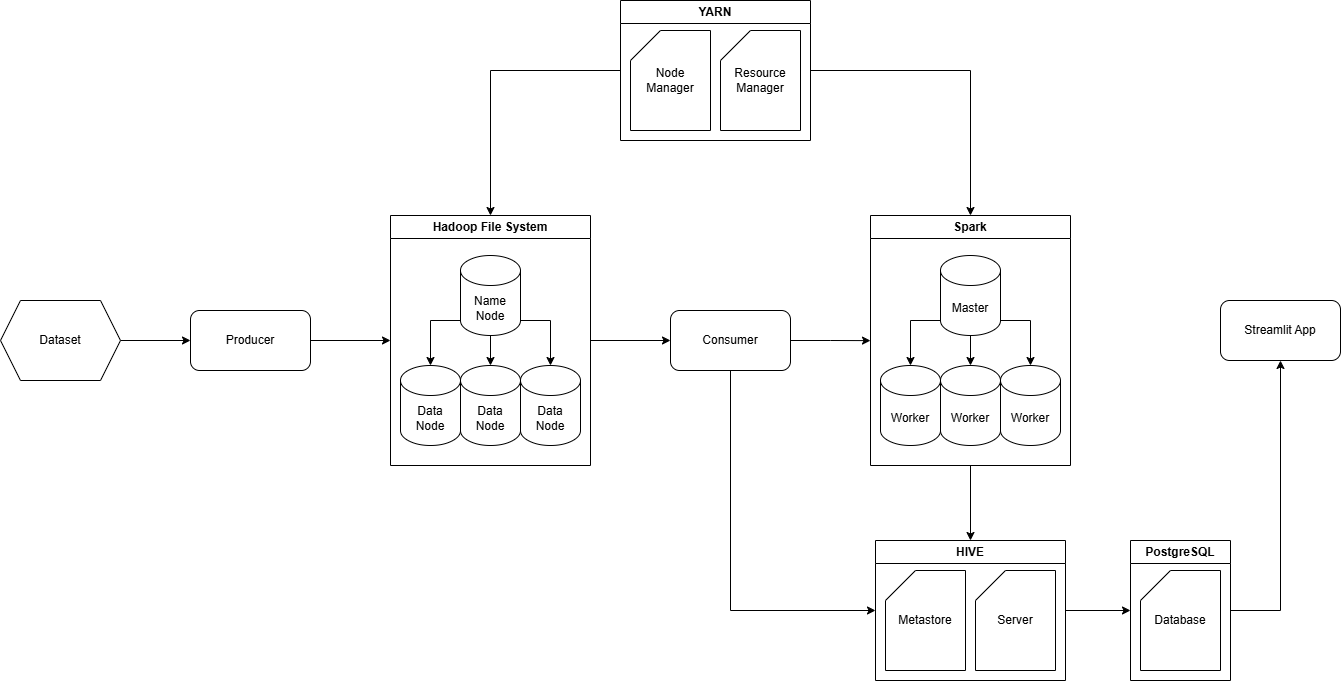
\includegraphics[width=\textwidth]{Diagrama.png}
		\caption{Arquitectura general del sistema distribuido para optimización de inventarios y logística.}
	\end{figure}
	
	\subsection*{Descripción de componentes}
	\begin{itemize}
		\item \textbf{Data Producer:} Componente encargado de replicar y variar los datos originales del dataset base, aplicando pequeñas perturbaciones controladas (p. ej., fluctuaciones de ventas o clima). Escribe los resultados generados en el sistema distribuido \textbf{HDFS}, actuando como fuente continua de datos para las fases posteriores.
		
		\item \textbf{Data Consumer:} Nodo que lee los datos desde HDFS, los interpreta y limpia, eliminando inconsistencias o valores atípicos. Realiza operaciones de agregación y normalización, guardando los resultados en la base de datos de PostgreSQL a través de HIVE. Su procesamiento está basado en \textbf{Spark}.
		
		\item \textbf{Streamlit:} Interfaz visual que se conecta a la base de datos para mostrar resultados, métricas y predicciones. Ofrece paneles de control con gráficos dinámicos, indicadores de stock y alertas de reposición, permitiendo al usuario interactuar en tiempo real con los datos.
		
		\item \textbf{Hadoop File System:} Conjunto de nodos de almacenamiento y un nodo maestro, que representan la infraestructura del sistema de archivos de Hadoop.
		
		\item \textbf{YARN:} Conjunto de contenedores con software encargado de distribuir los recursos del sistema para realizar procesos.
		
		\item \textbf{Spark:} Componente que realiza los trabajos distribuidos. El consumer se ejecuta sobre este componente.
		
		\item \textbf{HIVE:} Componente intermediaria entre el output del consumer y la base de datos. Realiza consultas y almacena datos sobre la base de datos de PostgreSQL
		
		\item \textbf{PostgreSQL:} Base de datos del sistema. Streamlit carga los datos a través de ella.
		
		
	\end{itemize}
	
\end{document}
